\section{Описание предметной области}

\subsection{Протокол сериализации Protocol Buffers}

Protocol Buffers --- протокол сериализации (передачи) структурированных данных, предложенный Google как эффективная бинарная альтернатива текстовому формату XML. Разработчики сообщают \cite{protobuf_doc}, что Protocol Buffers проще, компактнее и быстрее, чем XML, поскольку осуществляется передача бинарных данных, оптимизированных под минимальный размер сообщения.

По замыслу разработчиков, сначала должна быть описана структура данных (в формате protobuf), которая затем путём кодогенерации компилируется в классы на целевом языке программирования. Вместе с классами идёт код их сериализации в компактном формате представления. Чтение и запись данных доступна в высокоуровневых языках программирования --- таких как Java, C++ или Python.

На изображении \ref{fig:protobuf_algo} изображен алгоритм работы с протоколом \cite{protobuf_doc}.
\begin{figure}[ht]
    \centering
    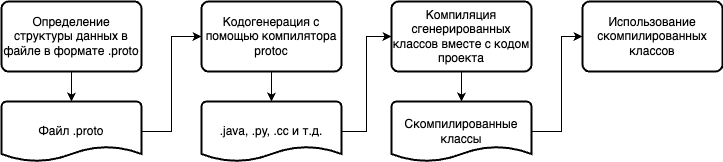
\includegraphics[width=0.85\linewidth]{\commonSecPathPrefix/sec_protobuf_sescription_attachments/protobuf_pipeline.drawio.png}
    \caption{Алгоритм работы разработчика с протоколом}
    \label{fig:protobuf_algo}
\end{figure}

К плюсам протокола относятся:

\begin{itemize}
    \item компактность сериализованных данных;
    \item быстрая десериализация;
    \item поддержка большого количества популярных языков программирования;
\end{itemize}

В 2010 году бэкенд Twitter перешёл на Protocol Buffers. По заявлению разработчиков Twitter, база в триллион твитов на XML занимала бы десять петабайт вместо одного \cite{protobuf_twitter}.

По заявлениям Google, Protocol Buffers по сравнению с XML:
\begin{itemize}
    \item проще;
    \item от 3 до 10 раз меньше;
    \item от 20 до 100 раз быстрее;
    \item более однозначный;
    \item позволяет создавать классы, которые в дальнейшем легче использовать программно.
\end{itemize}

Protocol Buffers не предназначен для чтения пользователем и представляет собой двоичный формат. Для десериализации данных необходим отдельный .proto-файл, в котором определяется формат сообщения.

\subsection{Формат описания сообщений в формате protobuf}

Единица данных, инкапсулирующая в себе данные о некоторой сущности, в протоколе protobuf называется сообщением и представляет собой аналог класса в языках программирования \cite{protobuf_api}.
Пример объявления сообщения представлен в листинге \ref{code:proto_example}:

\begin{lstlisting}[label=code:proto_example, caption={Пример простейшего protobuf-сообщения}]
message Person {
  string name = 1;
  int32 id = 2;
  string email = 3;
}
\end{lstlisting}

Поле сообщения описывается в формате <<тип данных-название-идентификатор>>. Тип данных может быть одним из стандартных типов, перечислением, коллекцией, protobuf-структурой либо другим protobuf-сообщением.
Перечень стандартных типов протокола\cite{protopub_scalar} предствлен в таблице \ref{sec_proto_desc:table:fields_desc}:

\begin{longtable}{
    | >{\raggedright\arraybackslash}m{0.100\textwidth}
    | >{\raggedright\arraybackslash}m{0.100\textwidth}
    | >{\raggedright\arraybackslash}m{0.140\textwidth}
    | >{\raggedright\arraybackslash}m{0.120\textwidth}
    | >{\raggedright\arraybackslash}m{0.100\textwidth}
    | >{\raggedright\arraybackslash}m{0.120\textwidth}
    | >{\raggedright\arraybackslash}m{0.140\textwidth}
    |}
    
    \caption{Соответствие встроенных типов протокола Protocol buffers типам в популярных языках программирования}
    \label{sec_proto_desc:table:fields_desc} \\
    \hline
    \centering\arraybackslash Proto & 
    \centering\arraybackslash C++ & 
    \centering\arraybackslash Java / Kotlin & 
    \centering\arraybackslash Python & 
    \centering\arraybackslash Go & 
    \centering\arraybackslash Ruby & 
    \centering\arraybackslash C\# \\
    \hline
    \endfirsthead

    \continueTableCaption \\
    \hline
    \centering\arraybackslash Proto & 
    \centering\arraybackslash C++ & 
    \centering\arraybackslash Java / Kotlin & 
    \centering\arraybackslash Python & 
    \centering\arraybackslash Go & 
    \centering\arraybackslash Ruby & 
    \centering\arraybackslash C\# \\
    \hline
    \endhead

    double & double & double & float & float64 & Float & double \\
    \hline
    float & float & float & float & float32 & Float & float \\
    \hline
    int32 & int32 & int & int & int32 & Fixnum or Bignum & int \\
    \hline
    int64 & int64 & long & int / long[4] & int64 & Bignum & long \\
    \hline
    uint32 & uint32 & int[2] & int / long[4] & uint32 & Fixnum / Bignum & uint \\
    \hline
    uint64 & uint64 & long[2] & int / long[4] & uint64 & Bignum & ulong \\
    \hline
    sint32 & int32 & int & int & int32 & Fixnum / Bignum & int \\
    \hline
    sint64 & int64 & long & int / long[4] & int64 & Bignum & long \\
    \hline
    fixed32 & uint32 & int[2] & int / long[4] & uint32 & Fixnum / Bignum & uint \\
    \hline
    fixed64 & uint64 & long[2] & int / long[4] & uint64 & Bignum & ulong \\
    \hline
    sfixed32 & int32 & int & int & int32 & Fixnum / Bignum & int \\
    \hline
    sfixed64 & int64 & long & int / long[4] & int64 & Bignum & long \\
    \hline
    bool & bool & boolean & bool & bool & TrueClass / FalseClass & bool \\
    \hline
    string & string & String & str / unicode[5] & string & String & string \\
    \hline
    bytes & string & ByteString & str / bytes & []byte & String & ByteString \\
    \hline

\end{longtable}

\subsection{Алгоритмы сериализации целых чисел, применяемые в протоколе}
Для кодирования целочисленных данных протокол использует формат \textit{varint}\cite{protobuf_habr}. 
Число в формате varint (int32 и int64) кодируется в последовательность байт, в которой у всех байт, кроме последнего, старший бит (MSB) выставляется в 1.
При преобразовании в стандартное представление старший бит каждого байта отбрасывается, а оставшиеся 7-битные составляющие соединяются друг с другом в обратном порядке. Формат восьмиразрядного varint был выбран для уменьшения размера пакета при передаче небольших чисел. Так, если число меньше 128, то оно будет занимать лишь 1 байт. Однако, числа близкие к максимально возможным, будут занимать больше места, чем в обычном формате. Например, максимальное значение, которое можно сохранить в 8-ми байтах, в формате varint — 10 байт. Отрицательные числа в формате varint всегда занимают наибольший размер, в зависимости от типа, поскольку старший бит у знакового числа выставлен в 1.

Проблема кодирования отрицательных чисел была решена использованием алгоритма ZigZag (sint32 и sint64), суть которого сводится в переносе бита знака из старшего разряда в младший. Кодирование алгоритмом ZigZag предполагает, что положительные и отрицательные числа будут чередоваться друг с другом с увеличением закодированного значения. В таком случае чётные числа будут положительными, а нечётные --- отрицательными.

Пусть value --- исходное значение, а N --- разрядность типа данных исходного значения, а encoded\_value --- закодированное алгоритмом ZigZag значение, тогда кодирование можно записать с помощью выражения на языке Си:

\begin{lstlisting}
encoded_value = (value << 1) ^ (value >> (N - 1));
\end{lstlisting}

Следует учесть, что вторая операция сдвига является арифметическим сдвигом, то есть при сдвиге вправо отрицательного числа старшие биты заполняются единицами, а не нулями (сдвиг знакового бита).

Декодирование выполняется более сложным способом: выполняется исключающее ИЛИ над закодированным значением, сдвинутым на 1 вправо для удаления знакового бита, и знаковым битом, полученным из закодированного числа, спроецированным на все биты через умножение на максимальное значение для N разрядов. Таким образом, знаковый бит переносится из младшего разряда в старший:

\begin{lstlisting}
uvalue = ((encoded_value & 1) * MAX_VALUE(N)) ^ (encoded_value >> 1);
\end{lstlisting}

Значение MAX\_VALUE(N) соответствует значению с N разрядами, заполненными единицами (например, 0xffffffff при N=32). Таким образом, умножение младшего бита, установленного в 1, на это число будет соответствовать значению −1 в знаковом типе данных. В языке Си декодирование необходимо осуществлять для значений encoded\_value и uvalue беззнакового типа, а затем значение uvalue должно преобразовываться в знаковый тип, не меняя битовое представление.

Все числовые значения, кроме fixed64, sfixed64 и double, в протоколе кодируются в формате varint.

\subsection{Алгоритм сериализации}

В общем виде формат представляет собой закодированную последовательность полей, состоящих из ключа и значения. В качестве ключа выступает номер, определённый для каждого поля сообщения в proto-файле \cite{proto_encoding}. Перед каждым полем указываются совместно закодированные номер поля в формате varint и тип поля. Если в качестве типа указана строка (string), вложенное сообщение, повторяющееся сообщение или набор байт (bytes), то следом идёт размер данных в формате varint. Далее идёт значение, соответствующее полю (данные).

Рассмотрим сериализацию сообщений в протоколе на практическом примере. Объявим в файле \textit{addressbook.proto} следующую структуру данных:

\begin{lstlisting}
syntax = "proto2";

message Person {
  optional string name = 1;
  optional int32 id = 2;
  optional string email = 3;

  enum PhoneType {
    MOBILE = 0;
    HOME = 1;
    WORK = 2;
  }

  message PhoneNumber {
    optional string number = 1;
    optional PhoneType type = 2 [default = HOME];
  }

  repeated PhoneNumber phones = 4;
}

message AddressBook {
  repeated Person people = 1;
}
\end{lstlisting}

Далее опишем код на C++, осуществляющий работу с данными сообщениями:

\begin{lstlisting}
#include <iostream>
#include <fstream>
#include <string>
#include "addressbook.pb.h"
using namespace std;
#define READ_EXAMPLE 1
#define WRITE_EXAMPLE 2
#define TYPE_EXAMPLE WRITE_EXAMPLE

// This function fills in a Person message based on user input.
void PromptForAddress(tutorial::Person* person) {
    cout << "Enter person ID number: ";
    int id;
    cin >> id;
    person->set_id(id);
    cin.ignore(256, '\n');

    cout << "Enter name: ";
    getline(cin, *person->mutable_name());

    cout << "Enter email address (blank for none): ";
    string email;
    getline(cin, email);
    if (!email.empty()) {
        person->set_email(email);
    }

    while (true) {
        cout << "Enter a phone number (or leave blank to finish): ";
        string number;
        getline(cin, number);
        if (number.empty()) {
            break;
        }

        tutorial::Person::PhoneNumber* phone_number = person->add_phones();
        phone_number->set_number(number);

        cout << "Is this a mobile, home, or work phone? ";
        string type;
        getline(cin, type);
        if (type == "mobile") {
            phone_number->set_type(tutorial::Person::MOBILE);
        }
        else if (type == "home") {
            phone_number->set_type(tutorial::Person::HOME);
        }
        else if (type == "work") {
            phone_number->set_type(tutorial::Person::WORK);
        }
        else {
            cout << "Unknown phone type.  Using default." << endl;
        }
    }

}

// Iterates though all people in the AddressBook and prints info about them.
void ListPeople(const tutorial::AddressBook& address_book) {
    for (int i = 0; i < address_book.people_size(); i++) {
        const tutorial::Person& person = address_book.people(i);

        cout << "Person ID: " << person.id() << endl;
        cout << "  Name: " << person.name() << endl;
        if (person.has_email()) {
            cout << "  E-mail address: " << person.email() << endl;
        }

        for (int j = 0; j < person.phones_size(); j++) {
            const tutorial::Person::PhoneNumber& phone_number = person.phones(j);

            switch (phone_number.type()) {
            case tutorial::Person::MOBILE:
                cout << "  Mobile phone #: ";
                break;
            case tutorial::Person::HOME:
                cout << "  Home phone #: ";
                break;
            case tutorial::Person::WORK:
                cout << "  Work phone #: ";
                break;
            }
            cout << phone_number.number() << endl;
        }
    }
}


// Main function:  Reads the entire address book from a file,
//   adds one person based on user input, then writes it back out to the same
//   file.
int main(int argc, char* argv[]) {
    // Verify that the version of the library that we linked against is
    // compatible with the version of the headers we compiled against.
    GOOGLE_PROTOBUF_VERIFY_VERSION;

    if (argc != 2) {
        cerr << "Usage:  " << argv[0] << " ADDRESS_BOOK_FILE" << endl;
        return -1;
    }

    tutorial::AddressBook address_book;

#if(TYPE_EXAMPLE == WRITE_EXAMPLE)
    {
        // Read the existing address book.
        fstream input(argv[1], ios::in | ios::binary);
        if (!input) {
            cout << argv[1] << ": File not found.  Creating a new file." << endl;
        }
        else if (!address_book.ParseFromIstream(&input)) {
            cerr << "Failed to parse address book." << endl;
            return -1;
        }
    }

    // Add an address.
    PromptForAddress(address_book.add_people());
    PromptForAddress(address_book.add_people());

    {
        // Write the new address book back to disk.
        fstream output(argv[1], ios::out | ios::trunc | ios::binary);
        if (!address_book.SerializeToOstream(&output)) {
            cerr << "Failed to write address book." << endl;
            return -1;
        }
    }

#elif(TYPE_EXAMPLE == READ_EXAMPLE)

    {
        // Read the existing address book.
        fstream input(argv[1], ios::in | ios::binary);
        if (!address_book.ParseFromIstream(&input)) {
            cerr << "Failed to parse address book." << endl;
            return -1;
        }
    }

    ListPeople(address_book);

#endif
    // Optional:  Delete all global objects allocated by libprotobuf.
    google::protobuf::ShutdownProtobufLibrary();

    return 0;
}
\end{lstlisting}

Запустим программу и заполним телефонную книгу двумя контактами:

\begin{lstlisting}
Enter person ID number: 170
Enter name: name1
Enter email address (blank for none): mail1
Enter a phone number (or leave blank to finish): 1234567
Is this a mobile, home, or work phone? mobile
Enter a phone number (or leave blank to finish):
Enter person ID number: 85
Enter name: name2
Enter email address (blank for none): mail2
Enter a phone number (or leave blank to finish): 7654321
Is this a mobile, home, or work phone? mobile
Enter a phone number (or leave blank to finish):
\end{lstlisting}

Идентификаторы, равные 170 и 85 выбраны для удобства: в шестнадцатиричном представлении они выглядят как \textit{AA} и \textit{55} соответственно, что облегчает просмотр бинарных данных.
Рассмотрим получившееся бинарное представление:

В результате работы программы получим бинарное представление, представленное на рисунке \ref{fig:encoded_proto}
\begin{figure}[ht]
    \centering
    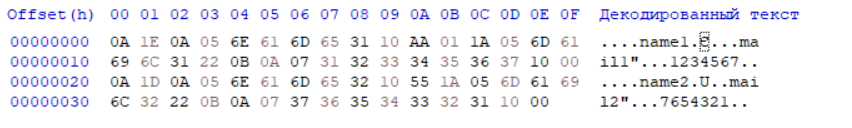
\includegraphics[width=0.85\linewidth]{\commonSecPathPrefix/sec_protobuf_sescription_attachments/encoded_proto.png}
    \caption{Сериализованное сообщение}
    \label{fig:encoded_proto}
\end{figure}

В protobuf данные хранятся по принципу ключ-значение. Ключ определяется по формуле \ref{sec_proto_desc:eq:proto_key}:
\begin{equation}
    \label{sec_proto_desc:eq:proto_key}
    (fieldNumber < < 3) | wireType
\end{equation}
\begin{explanationx}
\item [где] $ fieldNumber $ --- номер у переменной в описании структуры данных в файле *.proto;
\item       $ wireType $ --- значение, определяемое таблицей \ref{sec_proto_desc:table:wire_type_value}.
\end{explanationx}
\begin{longtable}{
    | >{\raggedright\arraybackslash}m{0.300\textwidth}
    | >{\raggedright\arraybackslash}m{0.300\textwidth}
    | >{\raggedright\arraybackslash}m{0.315\textwidth}
    |}
    
    \caption{Определение значения wireType}
    \label{sec_proto_desc:table:wire_type_value} \\
    \hline
    \centering\arraybackslash Значение wireType & 
    \centering\arraybackslash Описание данных & 
    \centering\arraybackslash Используется для типов \\
    \hline
    \endfirsthead

    \continueTableCaption \\
    \hline
    \centering\arraybackslash Значение wireType & 
    \centering\arraybackslash Описание данных & 
    \centering\arraybackslash Используется для типов \\
    \hline
    \endhead

    0 & Varint & int32, int64, uint32, uint64, sint32, sint64, bool, enum \\
    \hline
    1 & 64-битная переменная & fixed64, sfixed64, double \\
    \hline
    2 & Переменная длина & string, bytes, вложенные сообщения, repeated-поля \\
    \hline
    3 & Устаревшее, не используется & - \\
    \hline
    4 & Устаревшее, не используется & - \\
    \hline
    5 & 32-битная переменная & fixed32, sfixed32, float \\
    \hline

\end{longtable}

Воспользовавшись формулой \ref{sec_proto_desc:eq:proto_key} определим, какой ключ должен быть перед переменной id:
\begin{equation*}
    key = 2 << 3 | 0 = 0x10
\end{equation*}

Это же число видим в декодированом файле.

Определим ключ для переменной name типа string, воспользовавшись формулой \ref{sec_proto_desc:eq:proto_key}: 
\begin{equation*}
    1 << 3 | 2 = 0x0A
\end{equation*}

Заметим, что перед переменными name1 и name2 (0x04 и 0x24 байт) стоит не 0x0A а 0x05. Это основная особенность типов с переменной длиной. Для таких типов идёт сначала ключ, потом количество байт. 0x05 описывает количество байт на данную переменную. 


